\documentclass[11pt,a4paper]{article}
\usepackage[margin=2.3cm]{geometry}
\usepackage[T1]{fontenc}
\usepackage{lmodern}
\usepackage{amsmath,amssymb}
\usepackage{graphicx}
\usepackage{booktabs}
\usepackage{caption}
\usepackage[hidelinks]{hyperref}
\usepackage{cleveref}
\usepackage{xcolor}
\graphicspath{{../figures/}}
\newcommand{\todo}[1]{\textcolor{red}{[TODO: #1]}}
\newcommand{\ugm}{$\mu$g/m$^3$}

\title{A Machine-Learning Proxy for Black Carbon from Low-Cost Regulated-Pollutant and Meteorological Sensors}
\author{Jose Arias\\ \small Topics on Optimization and Machine Learning (TOML), UPC -- BarcelonaTECH}
\date{\todo{date} \quad --- \quad DRAFT v0}

\begin{document}
\maketitle

\begin{abstract}
Black carbon (BC) is a health-relevant pollutant that is not regulated, and measuring it is expensive. We build a BC proxy from co-located low-cost measurements of regulated pollutants (PM, NO$_x$, O$_3$, CO, SO$_2$), ultrafine particle counts and meteorology, using 4\,223 hourly samples from 2019. Forward subset selection with random forest keeps 7 of the 12 inputs: O$_3$, N\_CPC, PM$_1$, temperature, PM$_{10}$, humidity, and NO or CO. With a shuffled split, the FFNN ($R^2=0.78$, RMSE $=0.54$~\ugm) and gradient boosting ($R^2=0.78$) perform best, and all non-linear models clearly beat linear regression ($R^2=0.51$). With a temporal split (train January--September, test October--December), every non-linear model loses 0.07--0.14 in $R^2$. The best models are then the FFNN and kernel ridge regression ($R^2=0.67$), and gradient boosting drops the most. Shuffled evaluation therefore overestimates the accuracy of a deployed proxy.
\end{abstract}

%=====================================================================
\section{Introduction}
%=====================================================================
Black carbon (BC) is a major component of fine particulate matter. It is emitted by incomplete combustion, mainly from road traffic, and it is linked to cardiovascular and respiratory disease and to climate warming. Unlike PM$_{10}$, PM$_{2.5}$, NO$_2$ or O$_3$, BC is not regulated by the EU Air Quality Directives, and measuring it requires expensive instruments such as aethalometers. The proposal for a revised EU ambient air-quality directive (October 2022) calls for additional sampling points for unregulated pollutants of emerging concern, BC among them.

A \emph{proxy} is a virtual sensor that estimates a target pollutant from measurements of other variables. If BC can be estimated accurately from cheap sensors for regulated pollutants and meteorology, BC information can be obtained wherever such sensors exist. This report compares several non-linear regressors as BC proxies: support vector regression (SVR), random forest (RF), gradient boosting (GB) and a feed-forward neural network (FFNN), with $k$-nearest neighbours (KNN) and kernel ridge regression (KRR) as optional extras. It also addresses two practical questions. The first is which inputs are needed, which we answer with forward subset selection. The second is how much performance degrades when the model is trained in one season and applied in another (concept drift).

%=====================================================================
\section{Related work}
%=====================================================================
\todo{BC proxies in the literature: statistical and ML models from NO$_x$, PM, CO and meteorology; e.g.\ Fung et al.\ (J.\ Aerosol Sci., 2021) compare white-box and black-box models \cite{fung2021}. Add the course references on BC proxies in Barcelona.}
Tree ensembles~\cite{breiman2001,friedman2001} and kernel methods~\cite{drucker1997} are standard non-linear regressors for environmental data, and FFNNs are universal approximators~\cite{hornik1989}. When the data distribution changes between training and deployment (\emph{concept drift}~\cite{gama2014}), offline metrics computed on randomly shuffled data overestimate real-world performance.

%=====================================================================
\section{Methodology}
%=====================================================================
\paragraph{Models.} All models are trained on standardised inputs (scikit-learn pipelines). The model families are:
SVR with an RBF kernel ($C$, $\gamma$, $\epsilon$);
RF ($\max$ depth, minimum leaf size, fraction of features per split; 300 trees);
GB with squared loss ($n_{\text{estimators}}$, learning rate, depth; subsample 0.8);
FFNN (MLP with ReLU, Adam, early stopping; architecture and L2 penalty $\alpha$);
KNN ($k$, weighting) and KRR with an RBF kernel ($\alpha$, $\gamma$) as optional models;
MLR as a linear reference.

\paragraph{Feature selection.} We use greedy forward subset selection (FSS) with RF as the base learner, scoring each candidate subset by its cross-validated RMSE on the training set. We keep the smallest subset whose CV RMSE is within 1\% of the best. The selected subset is then fixed for every model, as the brief suggests.

\paragraph{Evaluation scenarios.}
\begin{itemize}
  \item \textbf{Shuffled}: a random 80/20 split, with 5-fold shuffled CV for tuning. Training and test samples come from the same seasons.
  \item \textbf{Temporal}: the first 80\% of the year for training and the last 20\% for testing, with 5-fold \texttt{TimeSeriesSplit} CV for tuning. The test period is unseen in time.
\end{itemize}
Hyperparameters are tuned by grid search inside the training set only. We report $R^2$, MAE and RMSE on the test set.

%=====================================================================
\section{Dataset}
%=====================================================================
The dataset contains 4\,223 hourly samples from 1 January to 10 December 2019. The target is BC (\ugm), and the 12 candidate inputs are the ultrafine particle number concentration (N\_CPC), PM$_{10}$, PM$_{2.5}$, PM$_1$, NO$_2$, O$_3$, SO$_2$, CO, NO, NO$_x$, temperature and relative humidity. No values are missing, but coverage is very uneven (\cref{fig:cov}): January--March and September--October contain 480--620 hours each, while May, June, November and December have fewer than 150. The timestamps are day-first (\texttt{dd/mm/yy}). The brief lists NO twice; the file actually contains NO$_2$ and NO.

BC is right-skewed: mean 1.31, median 0.97, maximum 12.8~\ugm. Its strongest linear correlations are with traffic and combustion tracers: N\_CPC (0.51), PM$_{2.5}$ and PM$_1$ (0.50), NO$_2$ (0.49) and NO$_x$ (0.47). Its correlation with O$_3$ is negative ($-0.35$), consistent with titration of O$_3$ by fresh NO emissions (\cref{fig:corr}). Temperature and humidity are almost uncorrelated with BC linearly. Several inputs are strongly collinear with each other (the PM fractions; NO, NO$_2$ and NO$_x$).

\begin{figure}[t]\centering
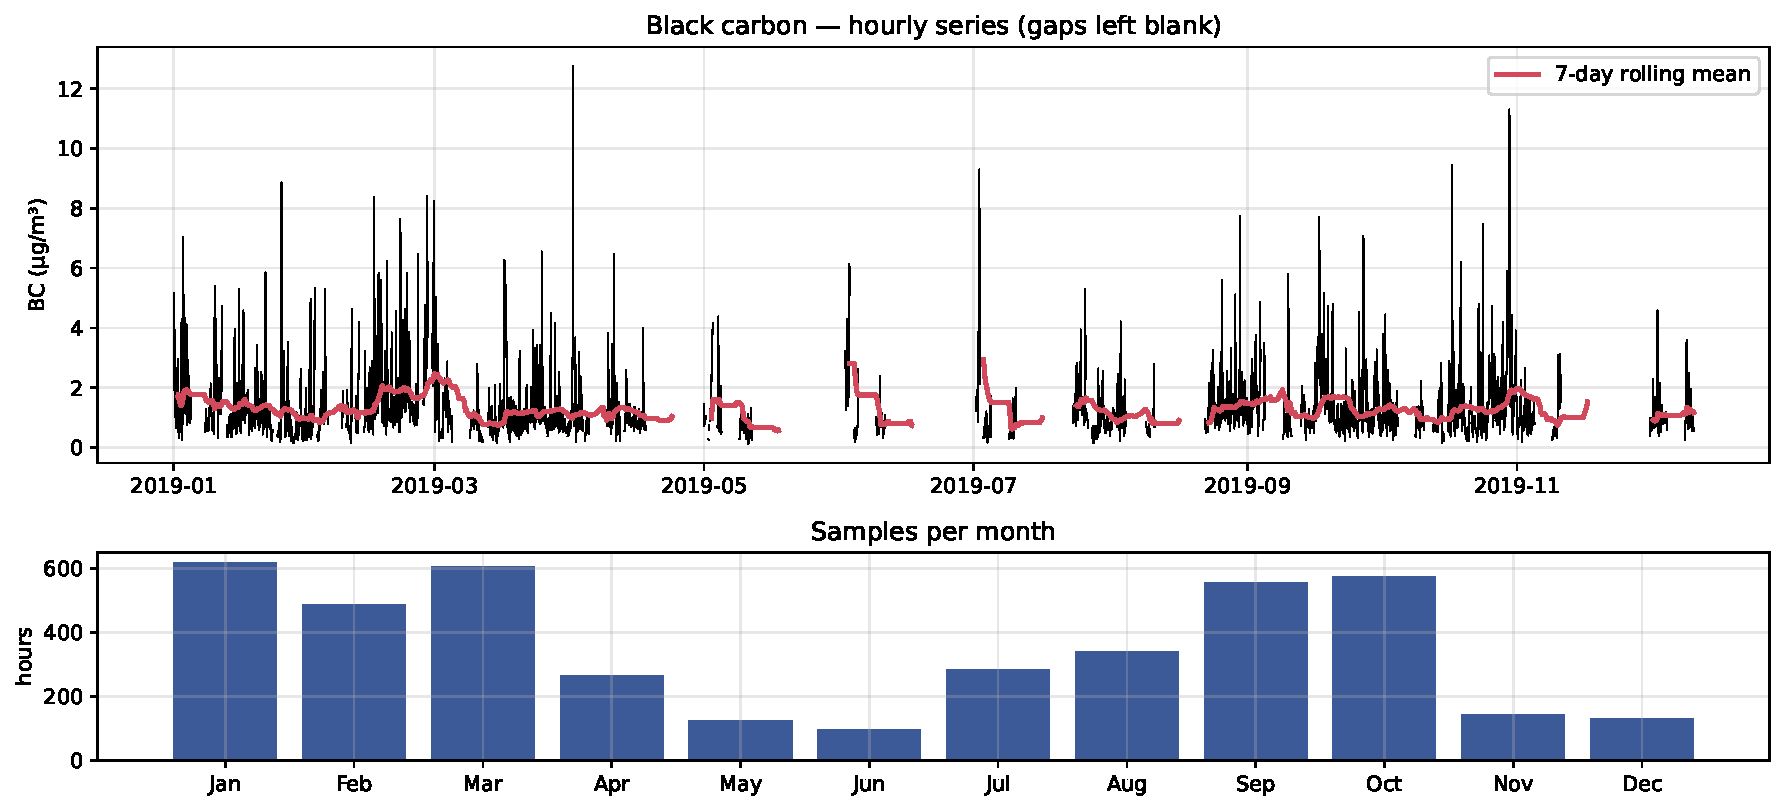
\includegraphics[width=\linewidth]{2_timeseries_coverage.pdf}
\caption{BC hourly series with a 7-day rolling mean (top) and the number of samples per month (bottom).}\label{fig:cov}
\end{figure}
\begin{figure}[t]\centering
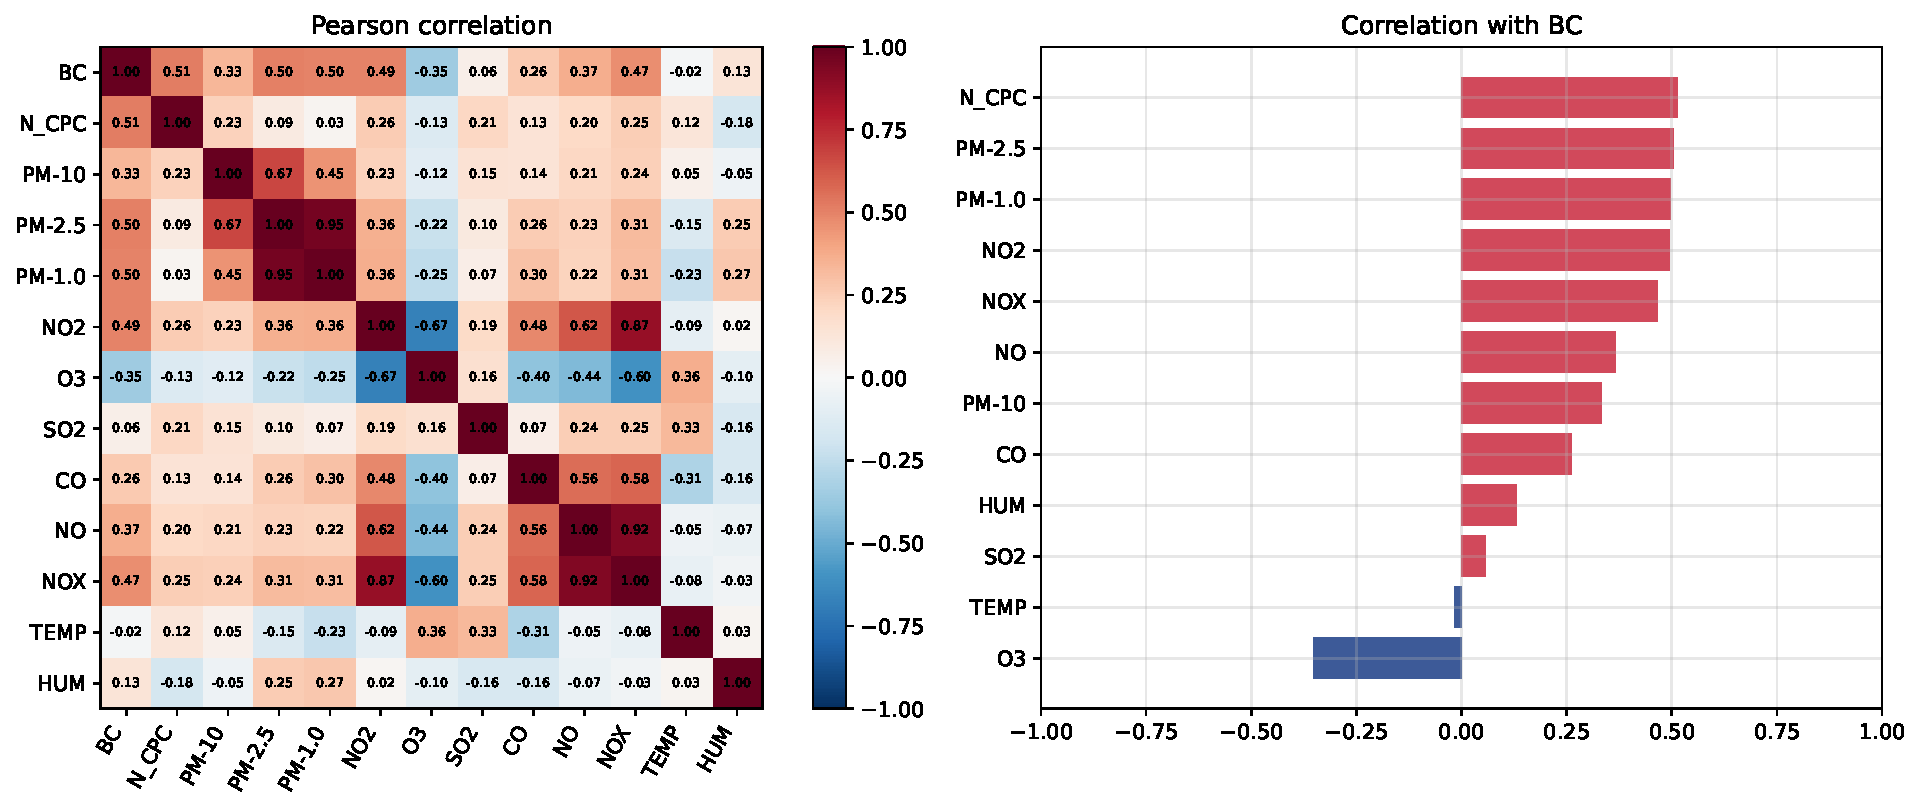
\includegraphics[width=\linewidth]{2_correlation.pdf}
\caption{Pearson correlation matrix (left) and correlation of each input with BC (right).}\label{fig:corr}
\end{figure}
\begin{figure}[t]\centering
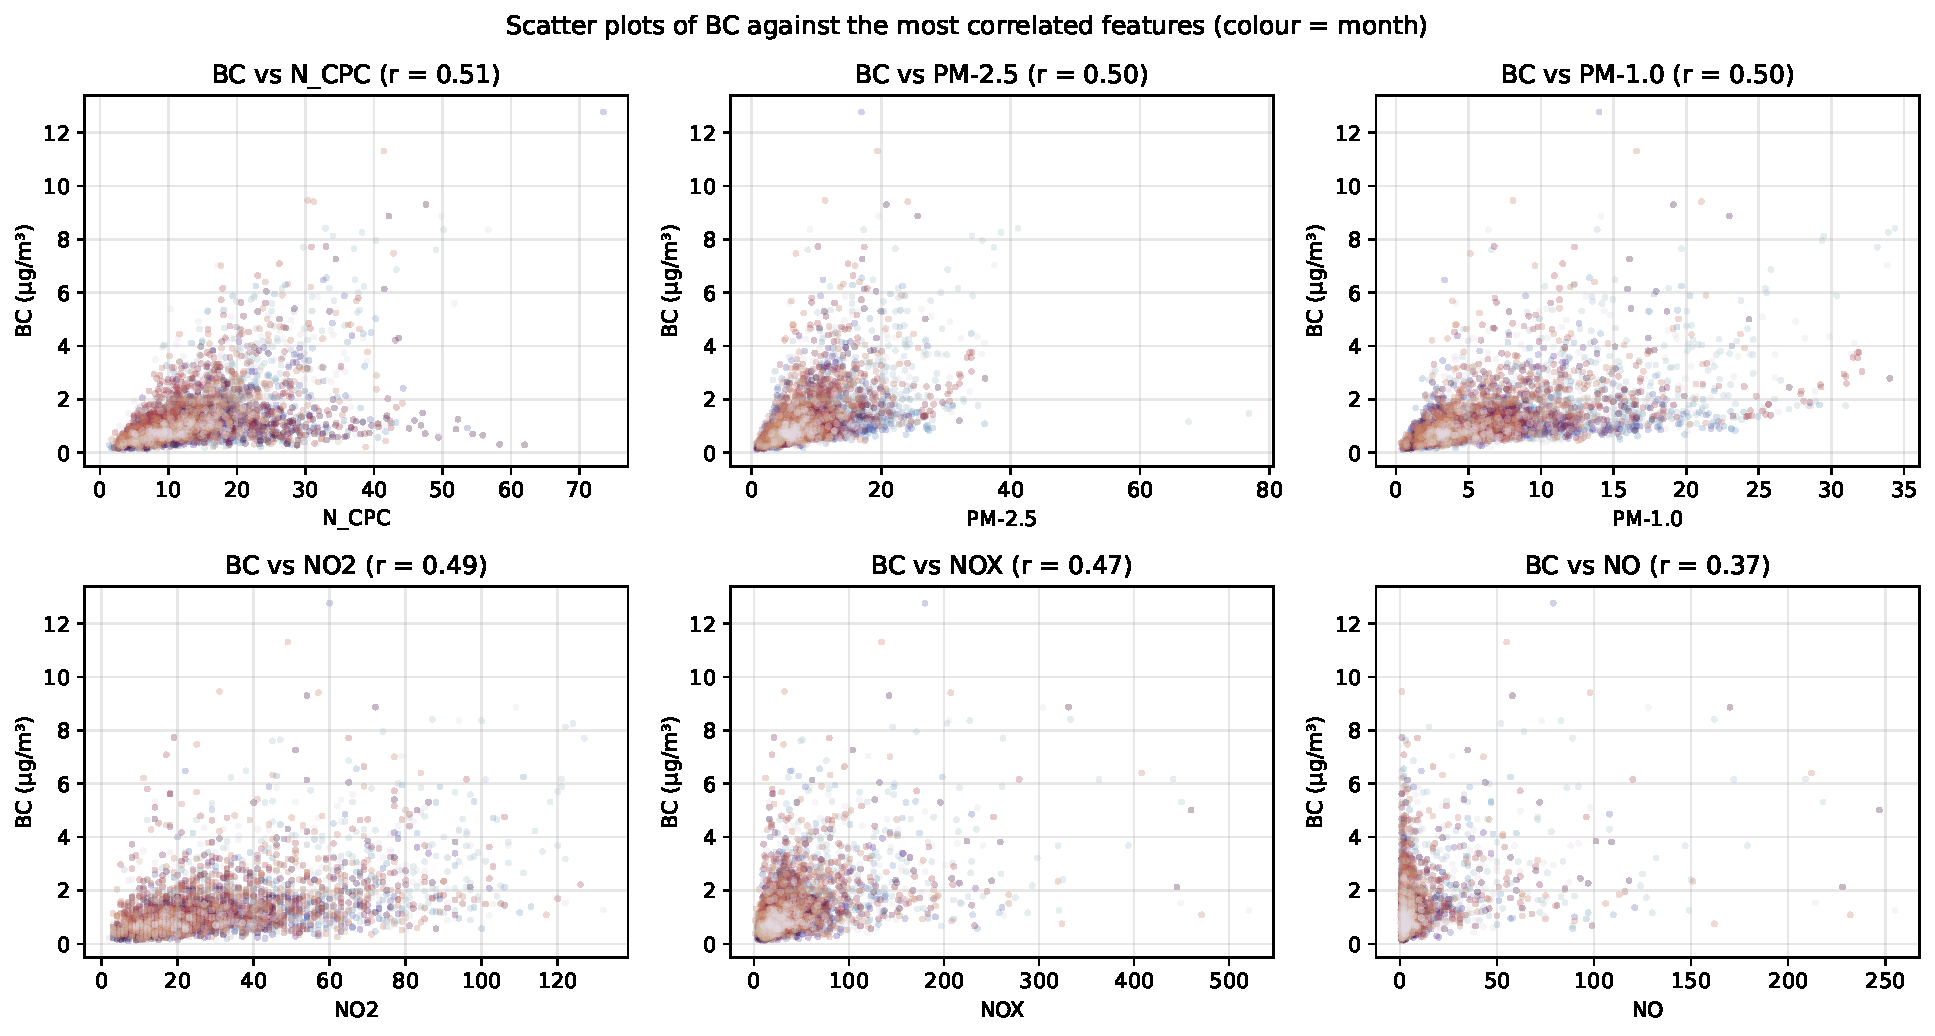
\includegraphics[width=\linewidth]{2_scatter.pdf}
\caption{BC against the six inputs most correlated with it (colour = month).}\label{fig:scat}
\end{figure}
\begin{figure}[t]\centering
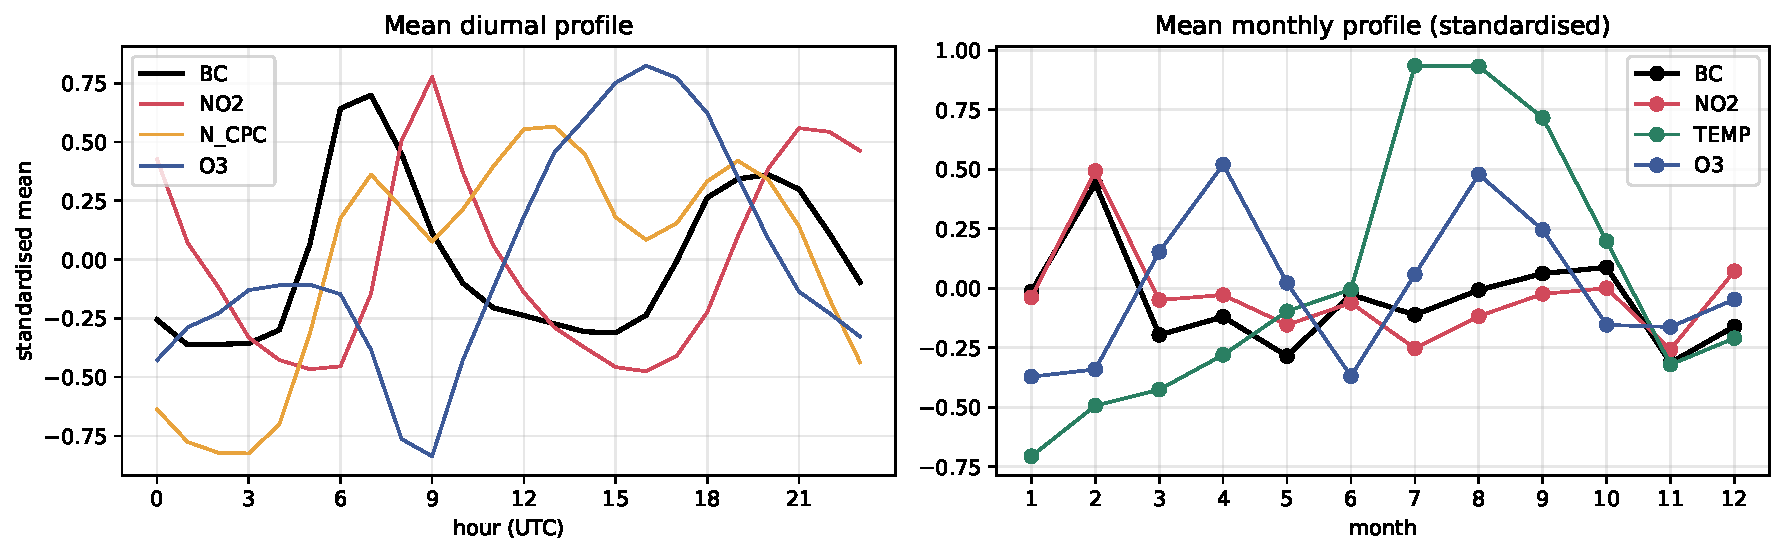
\includegraphics[width=\linewidth]{2_profiles.pdf}
\caption{Standardised mean diurnal (left) and monthly (right) profiles of BC and selected inputs.}\label{fig:prof}
\end{figure}

\paragraph{Splits.} Shuffled: 3\,378 training and 845 test samples, both spanning the whole year. Temporal: training from 1 January to 1 October (3\,378 samples), testing from 1 October to 10 December (845 samples). The mean BC is almost the same in both test sets (1.31 vs 1.29~\ugm), so any loss of performance in the temporal scenario comes from changes in the \emph{relation} between the inputs and BC, not from a shift in the BC level.

%=====================================================================
\section{Results}
%=====================================================================
\subsection{Feature selection}
\Cref{fig:fss} shows the FSS path. In both scenarios the first three features are O$_3$, N\_CPC and PM$_1$, and they reduce the CV RMSE from about 1.0 to 0.65--0.69~\ugm. Temperature comes fourth, and the remaining features each add very little. The 1\%-tolerance rule keeps 7 features in both scenarios: \{O$_3$, N\_CPC, PM$_1$, TEMP, NO, PM$_{10}$, HUM\} for the shuffled split and \{O$_3$, N\_CPC, PM$_1$, TEMP, PM$_{10}$, CO, HUM\} for the temporal one.

O$_3$ is selected first even though its linear correlation with BC is weak. A tree can use its non-linear relation with BC: very low O$_3$ indicates fresh NO emissions, and hence traffic. NO$_2$ and NO$_x$ are never selected despite having the highest linear correlations, because O$_3$ and the particle counts already carry the same information. \todo{verify this interpretation with a partial-dependence plot.} Beyond about 7 features the CV RMSE rises slightly, especially in the temporal scenario, which suggests overfitting to the conditions of the training period.

\begin{figure}[t]\centering
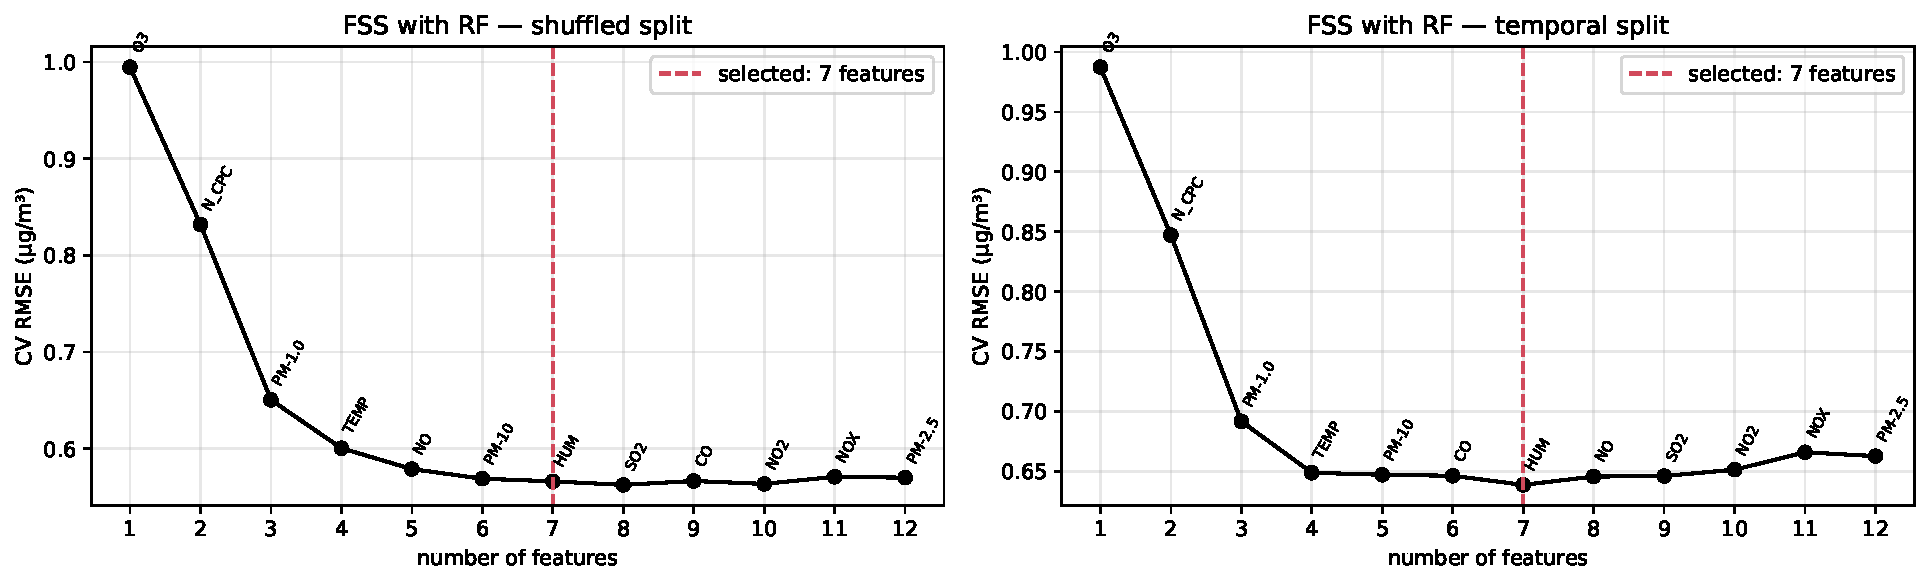
\includegraphics[width=\linewidth]{2_fss.pdf}
\caption{Forward subset selection with RF: CV RMSE vs number of features, with the feature added at each step.}\label{fig:fss}
\end{figure}

\subsection{Model comparison}
\begin{table}[h]
\centering
\caption{Test performance with the FSS-selected features (BC in \ugm).}\label{tab:res}
\begin{tabular}{lcccccc}
\toprule
 & \multicolumn{3}{c}{Shuffled split} & \multicolumn{3}{c}{Temporal split}\\
\cmidrule(lr){2-4}\cmidrule(lr){5-7}
Model & $R^2$ & MAE & RMSE & $R^2$ & MAE & RMSE\\
\midrule
MLR    & 0.513 & 0.503 & 0.808 & 0.521 & 0.460 & 0.774\\
SVR    & 0.736 & 0.351 & 0.594 & 0.638 & 0.374 & 0.673\\
RF     & 0.735 & 0.353 & 0.596 & 0.640 & 0.395 & 0.671\\
GBoost & 0.781 & \textbf{0.331} & 0.541 & 0.637 & 0.399 & 0.674\\
FFNN   & \textbf{0.782} & 0.333 & \textbf{0.540} & \textbf{0.669} & 0.407 & \textbf{0.644}\\
KNN    & 0.704 & 0.362 & 0.630 & 0.596 & 0.422 & 0.711\\
KRR    & 0.740 & 0.358 & 0.590 & 0.668 & \textbf{0.371} & 0.645\\
\bottomrule
\end{tabular}
\end{table}

\begin{table}[h]
\centering\small
\caption{Selected hyperparameters (grid search on the training set).}\label{tab:hp}
\begin{tabular}{lll}
\toprule
Model & Shuffled & Temporal\\
\midrule
SVR & $C=100,\gamma=0.03,\epsilon=0.2$ & $C=10,\gamma=0.03,\epsilon=0.2$\\
RF & depth none, leaf 1, max\_feat 0.66 & depth none, leaf 3, max\_feat 1.0\\
GBoost & 800 trees, lr 0.03, depth 5 & 300 trees, lr 0.03, depth 3\\
FFNN & (128, 64), $\alpha=0.01$ & (64), $\alpha=0.01$\\
KNN & $k=5$, distance & $k=10$, distance\\
KRR & $\alpha=0.01,\gamma=0.03$ & $\alpha=0.1,\gamma=0.03$\\
\bottomrule
\end{tabular}
\end{table}

\Cref{tab:res,fig:comp} compare the models. Every non-linear model improves on MLR by a wide margin: $R^2$ rises from 0.51 to 0.70--0.78 in the shuffled split. The relation between BC and its proxies is clearly non-linear. With shuffled data, the FFNN and GB are best ($R^2\approx0.78$), followed by KRR, SVR and RF, which form a group at about 0.74. KNN is the weakest non-linear model.

\begin{figure}[t]\centering
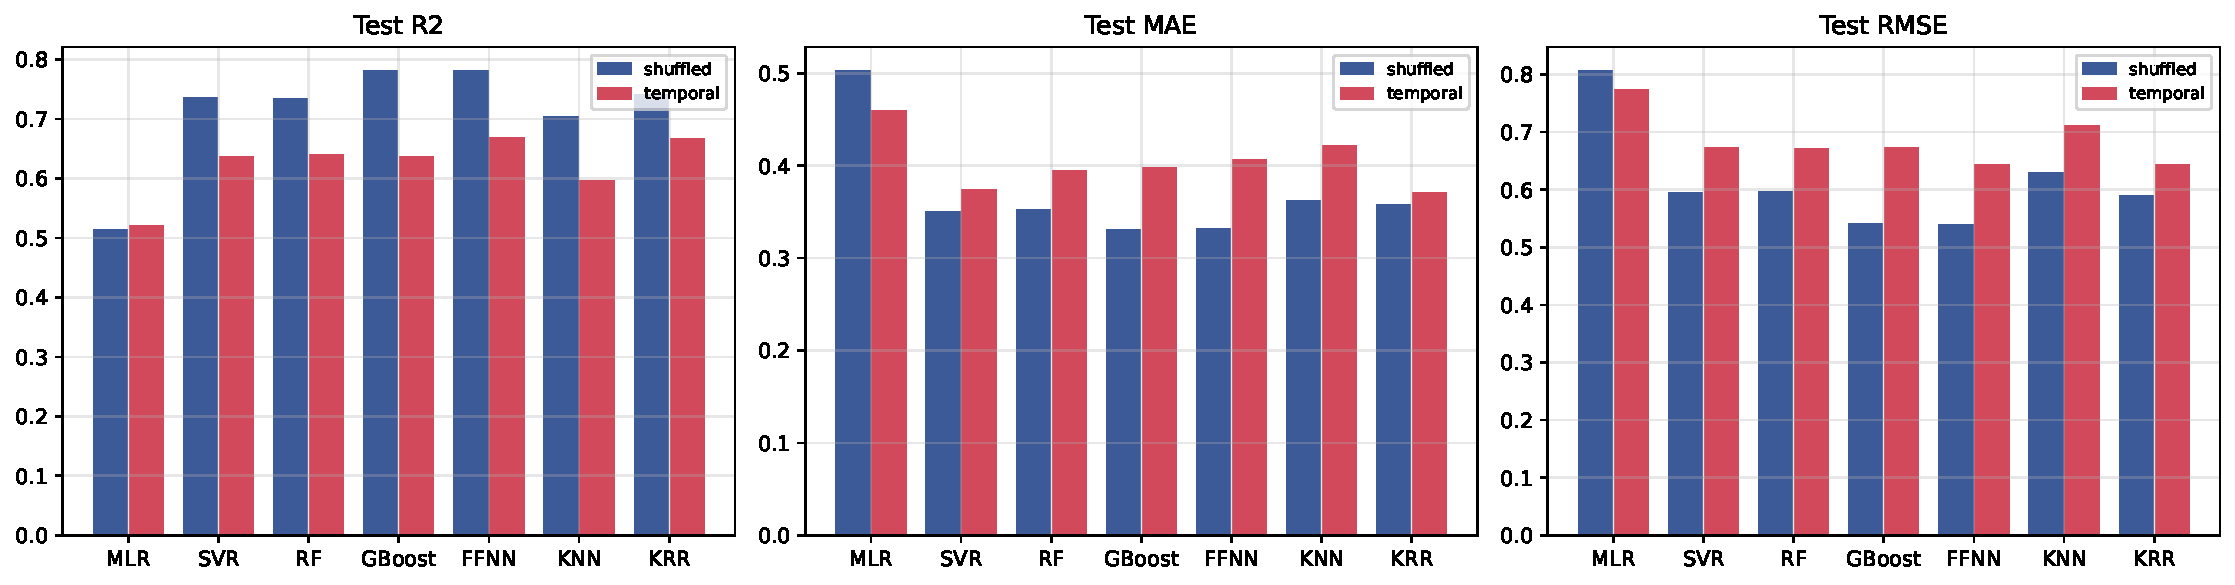
\includegraphics[width=\linewidth]{2_model_comparison.pdf}
\caption{Test $R^2$, MAE and RMSE of every model in the shuffled and temporal scenarios.}\label{fig:comp}
\end{figure}

\subsection{Hyperparameters}
\Cref{fig:hp} shows how the CV RMSE depends on the main hyperparameter of each model. In the temporal CV, every model prefers more regularisation: a lower $C$ for SVR, larger leaves for RF, shallower and fewer trees for GB, a smaller FFNN and a larger $k$ for KNN (\cref{tab:hp}). Validation folds that lie in the future penalise models that memorise conditions specific to the training period. The FFNN is insensitive to $\alpha$ up to about 1 and degrades sharply at $\alpha=10$. GB keeps improving slowly with more trees in the shuffled case, but not in the temporal case.

\begin{figure}[t]\centering
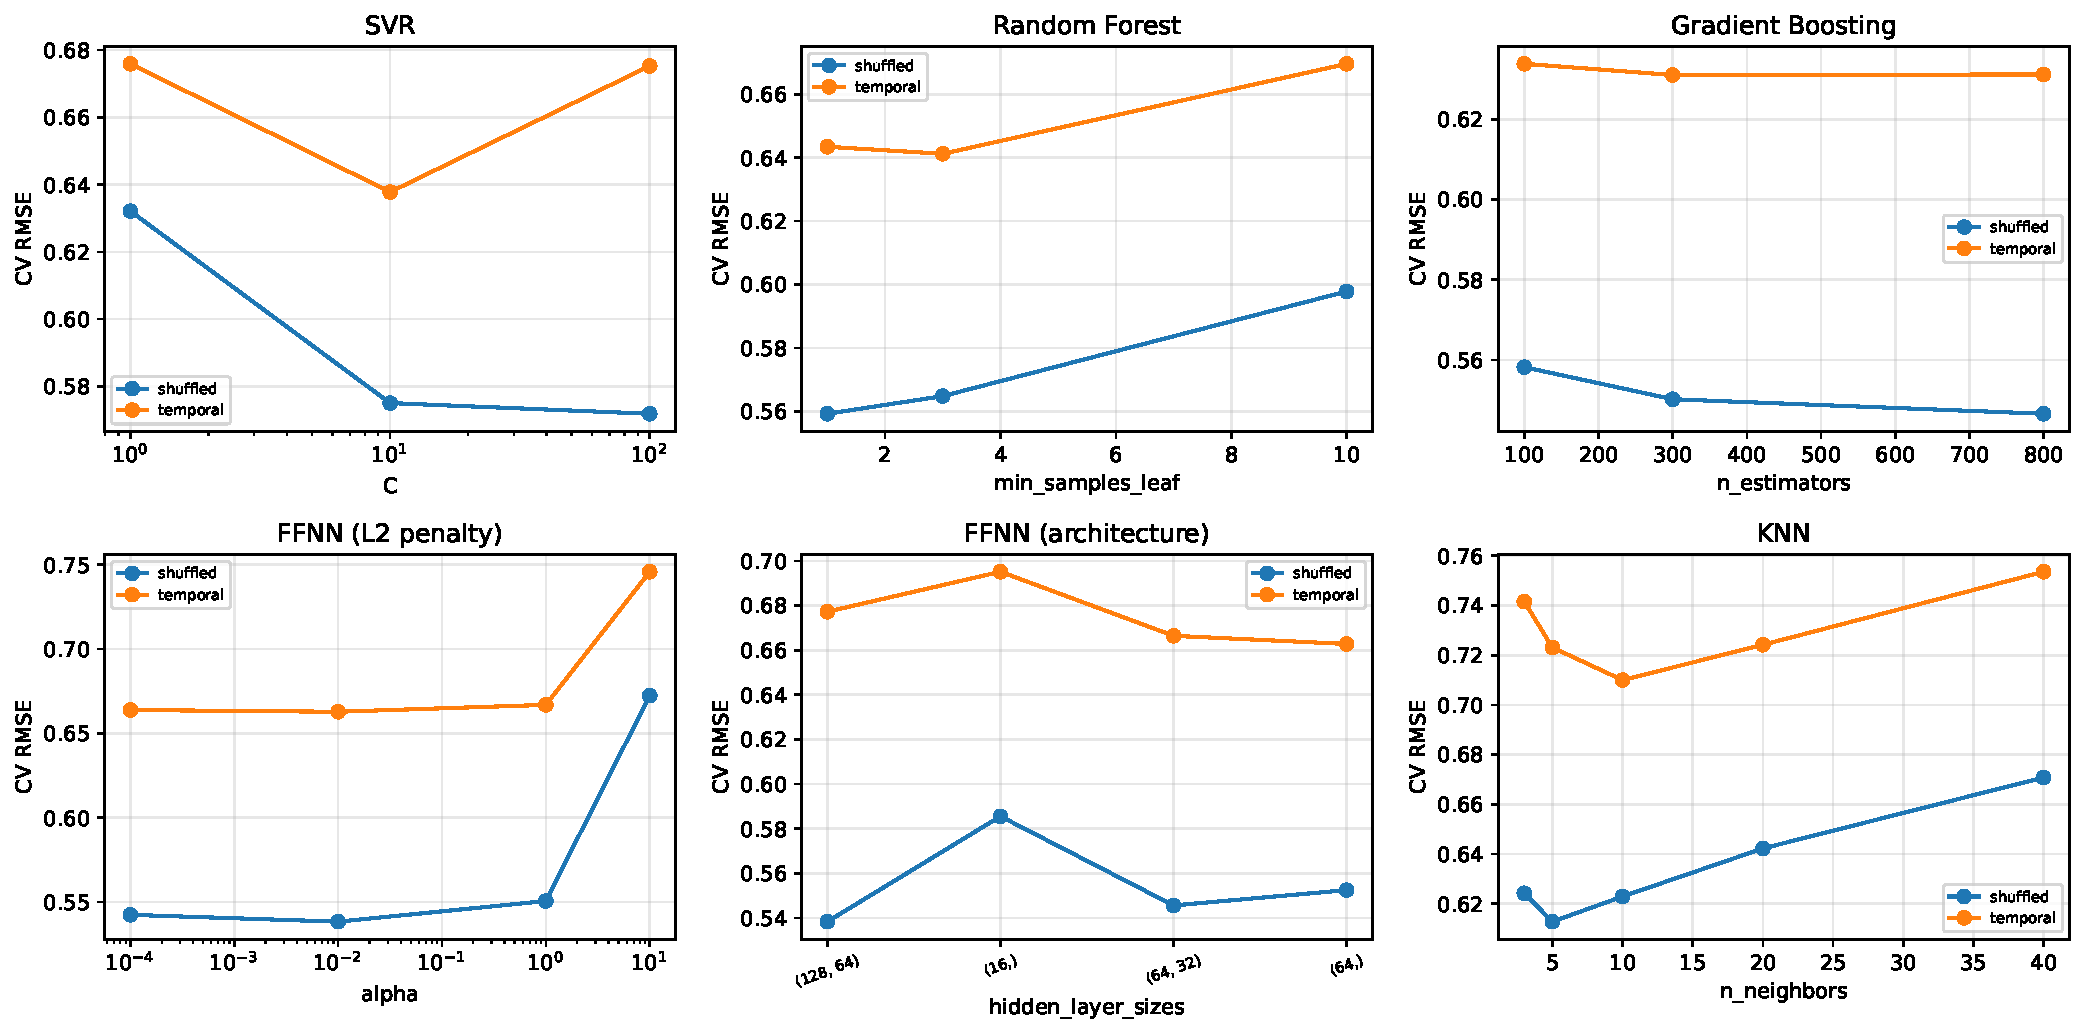
\includegraphics[width=\linewidth]{2_hyperparams.pdf}
\caption{CV RMSE vs the main hyperparameters (each point is the best over the other parameters of the grid) for both scenarios.}\label{fig:hp}
\end{figure}

\subsection{Shuffled vs temporal split: concept drift}
Every non-linear model performs worse on the temporal split, with $R^2$ losses of 0.07 (KRR) to 0.14 (GB). MLR is the exception and does not change ($0.51\to0.52$). The ranking also changes: GB falls from first to fifth, while KRR and the FFNN are the most robust. The most flexible models exploit, in the shuffled split, neighbouring hours of the same day that appear in both training and test sets. This information is not available when the test period lies entirely in the future. \Cref{fig:time,fig:best} show the predictions with the temporal order restored. The proxy follows the dynamics well, but it systematically underestimates the highest BC peaks (above about 5~\ugm), which are rare in the training data. In this dataset the drift is moderate because the training period already includes a winter. Training only on summer data would be a harsher test. \todo{optional extra experiment: train on Apr--Aug, test on Oct--Dec.}

\begin{figure}[t]\centering
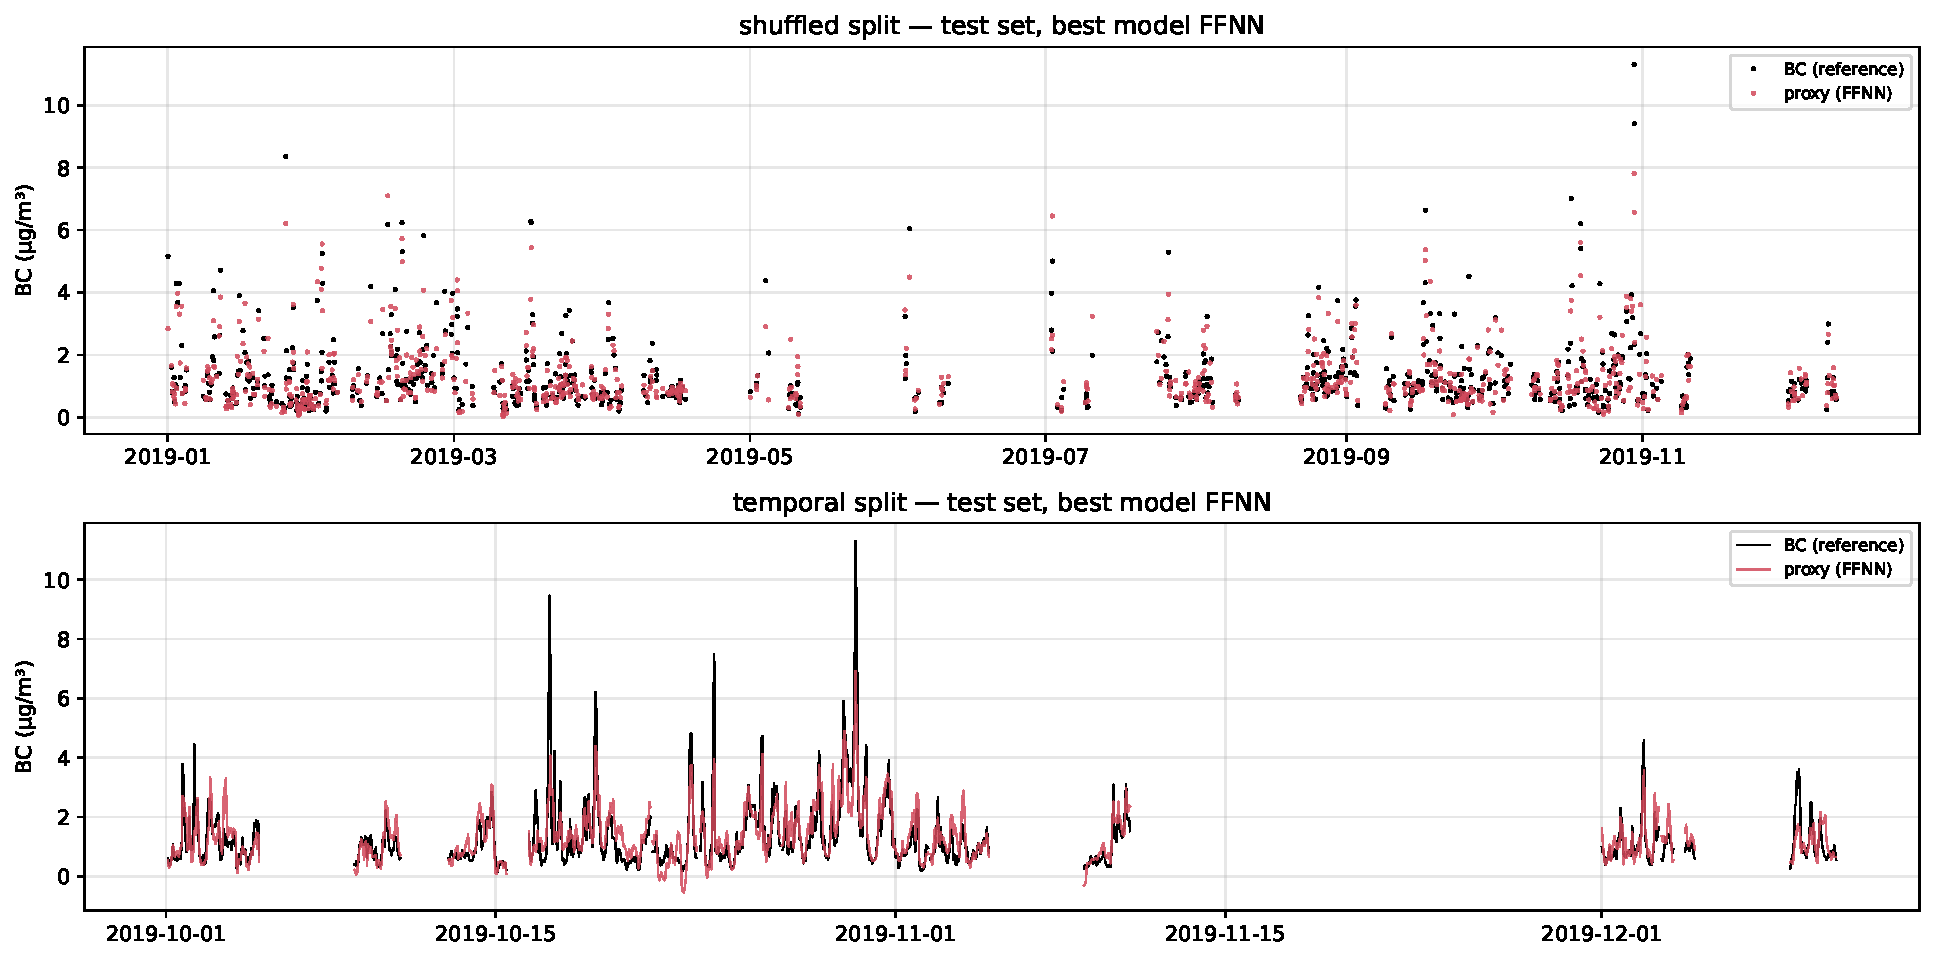
\includegraphics[width=\linewidth]{2_predictions_time.pdf}
\caption{Test-set predictions of the best model in time, for the shuffled (top) and temporal (bottom) splits.}\label{fig:time}
\end{figure}
\begin{figure}[t]\centering
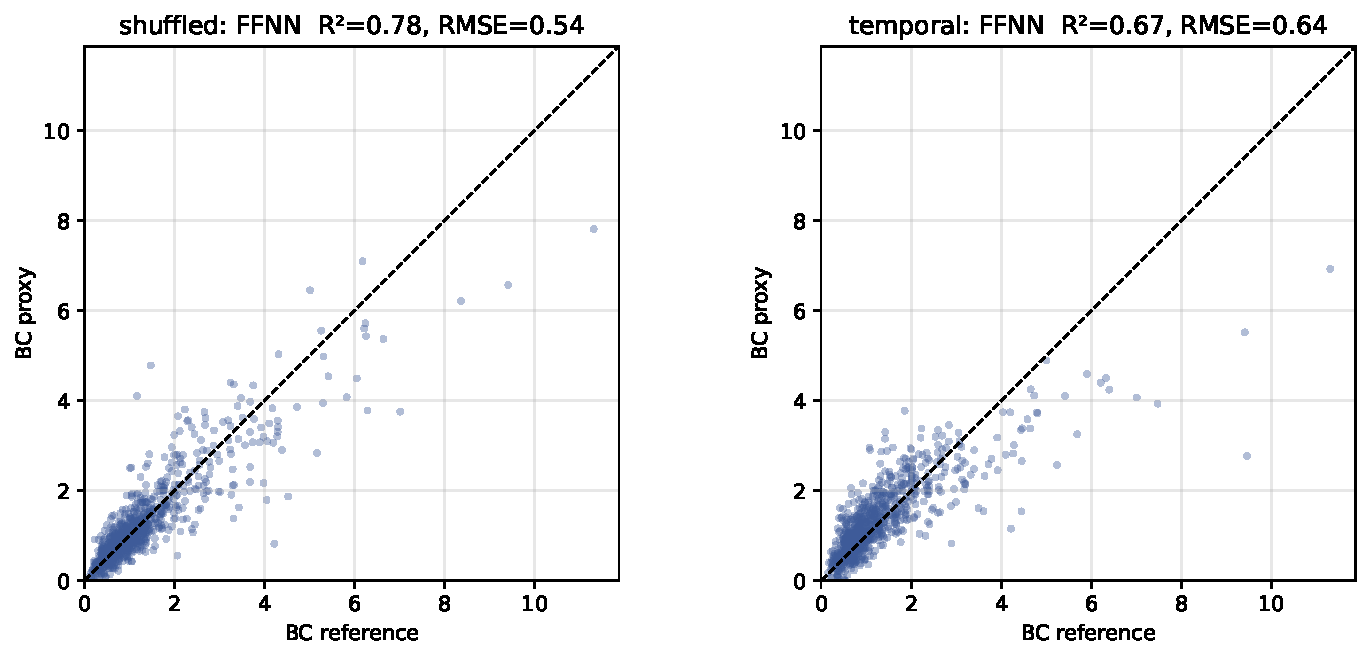
\includegraphics[width=0.8\linewidth]{2_scatter_best.pdf}
\caption{Proxy vs reference BC for the best model in each scenario.}\label{fig:best}
\end{figure}
\begin{figure}[t]\centering
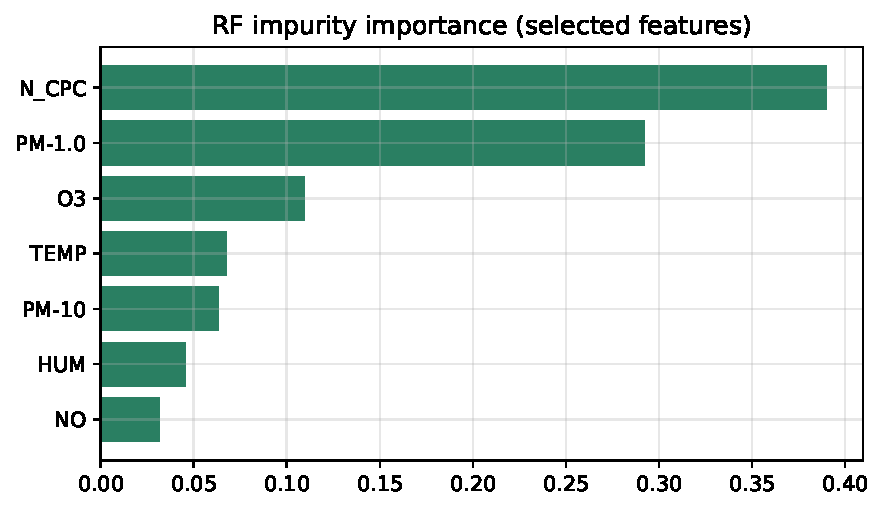
\includegraphics[width=0.55\linewidth]{2_importance.pdf}
\caption{RF impurity-based importance of the selected features (shuffled split).}\label{fig:imp}
\end{figure}

%=====================================================================
\section{Conclusions}
%=====================================================================
\begin{itemize}
  \item A BC proxy built from cheap regulated-pollutant and meteorological sensors explains up to 78\% of the hourly BC variance, compared with 51\% for a linear model. Non-linearity is essential.
  \item Seven inputs are enough. O$_3$, N\_CPC and PM$_1$ carry most of the information, and the NO$_x$ species are redundant once O$_3$ and particle counts are included.
  \item Shuffled evaluation overestimates deployed performance. With a temporal split, $R^2$ drops by 0.07--0.14, the optimal models are more regularised, and the most flexible model (GB) suffers the most. The FFNN and KRR are the most robust choices in this setting.
  \item \todo{limitations: one site, one year, uneven coverage; future work: log-transform of BC, lag/hour-of-day features, retraining strategies against drift.}
\end{itemize}

\begin{thebibliography}{99}\small
\bibitem{breiman2001} L.~Breiman, ``Random forests,'' \emph{Machine Learning}, vol.~45, pp.~5--32, 2001.
\bibitem{friedman2001} J.~H. Friedman, ``Greedy function approximation: a gradient boosting machine,'' \emph{Annals of Statistics}, vol.~29, no.~5, pp.~1189--1232, 2001.
\bibitem{drucker1997} H.~Drucker, C.~J.~C. Burges, L.~Kaufman, A.~Smola, V.~Vapnik, ``Support vector regression machines,'' in \emph{Advances in Neural Information Processing Systems 9}, 1997.
\bibitem{hornik1989} K.~Hornik, M.~Stinchcombe, H.~White, ``Multilayer feedforward networks are universal approximators,'' \emph{Neural Networks}, vol.~2, no.~5, pp.~359--366, 1989.
\bibitem{gama2014} J.~Gama, I.~\v{Z}liobait\.{e}, A.~Bifet, M.~Pechenizkiy, A.~Bouchachia, ``A survey on concept drift adaptation,'' \emph{ACM Computing Surveys}, vol.~46, no.~4, 2014.
\bibitem{fung2021} P.~L. Fung et al., ``Evaluation of white-box versus black-box machine learning models in estimating ambient black carbon concentration,'' \emph{Journal of Aerosol Science}, vol.~152, 2021. \todo{verify reference details}
\end{thebibliography}
\end{document}
